% --- IMPORTS ---
\documentclass[leqno]{article}
\usepackage{graphicx}
\usepackage{dsfont}
\usepackage{mathtools}
\usepackage{amssymb}
\usepackage{amsmath}
\usepackage{amsthm}
\usepackage{float}
\usepackage{ragged2e}
\usepackage{tensor}
\usepackage{fancyhdr}
\usepackage{empheq}
\usepackage[most]{tcolorbox}
\usepackage{enumitem}
\usepackage{dirtytalk}
\usepackage{marginnote}
\usepackage{microtype}
\usepackage[
  a4paper,
  left=0.8in,
  right=1in,
  top=1in,
  bottom=0.5in,
  headheight=14pt,
  headsep=0.4in
]{geometry}
\setlength{\parindent}{0cm}
% --- TikZ Packages ---
\usepackage{pgfplots}
\pgfplotsset{compat=1.18}
\usepgfplotslibrary{fillbetween, polar}
\usetikzlibrary{calc, positioning}
\usetikzlibrary{angles, quotes}
\usetikzlibrary{arrows.meta}
\usetikzlibrary{decorations.pathreplacing, decorations.markings}
\usetikzlibrary{patterns}
\usetikzlibrary{intersections}
% --- URL Packages ---
\usepackage[colorlinks=true,linkcolor=red,citecolor=magenta,urlcolor=black]{hyperref}%
\urlstyle{same}
% --- END OF IMPORTS ---

% --- CUSTOM COMMANDS ---
\RenewDocumentCommand{\marks}{o m}{%
  \IfValueTF{#1}%
    {\marginnote{\raggedright\textbf{[#2]}}[#1]}%
    {\marginnote{\raggedright\textbf{[#2]}}}%
}
\newcommand{\vspacerule}[2]{%
  \par\vspace*{#1}%
  \noindent\hrulefill\par
  \vspace*{#2}%
}
\definecolor{scarlet}{RGB}{205, 40, 75}
\newcommand{\questionitem}{%
  \item\phantomsection
  \addcontentsline{toc}{section}{Question \number\value{enumi}}%
}
\renewcommand{\contentsname}{Questions}
% --- END OF CUSTOM COMMANDS ---

% --- HEADER CONFIG ---
\pagestyle{fancy}
\fancyhead{}
\fancyfoot{}
\renewcommand{\headrulewidth}{0.9pt}
\lhead{Vector Momentum and Impulse}
\chead{}
\rhead{\href{https://danieljsmith.org}{danieljsmith.org}}
% --- END OF HEADER CONFIG ---

\begin{document}
\vspace*{20pt}
\tableofcontents
\newpage
\begin{enumerate}[
  label=\textbf{\arabic*.},
  leftmargin=*,
  topsep=0pt,
  partopsep=0pt,
  parsep=0pt
]


% ---- Question 1 ----
\questionitem
% [Source: _QBT__Vector_Momentum_and_Impulse, Q1]

A particle $P$ of mass $2\,\mathrm{kg}$ is moving with speed $15\,\mathrm{m\,s^{-1}}$ in the direction of $3\mathbf{i}+4\mathbf{j}$ when it receives an impulse $\mathbf{J}\,\mathrm{N\,s}$. Immediately after receiving the impulse, $P$ is moving with speed $17\,\mathrm{m\,s^{-1}}$ in the direction of $8\mathbf{i}+15\mathbf{j}$. \\

\begin{enumerate}[label=\textbf{(\alph*)}]
  \item Find the magnitude of $\mathbf{J}$ \marks{4} \\
\end{enumerate}
The angle between the direction of the impulse and the direction of motion of $P$ immediately before receiving the impulse is $\alpha^\circ$. \\
\begin{enumerate}[label=\textbf{(\alph*)}, resume]
  \item Find the value of $\alpha$ \marks{3} \\
\end{enumerate}

\newpage

% ---- Question 2 ----
\questionitem
% [Source: _QBT__Vector_Momentum_and_Impulse, Q2]

A particle $P$ of mass $0.8\,\mathrm{kg}$ is moving with velocity $\lambda(\mathbf{i}+2\mathbf{j})\,\mathrm{m\,s^{-1}}$ when $P$ receives an impulse of magnitude $\dfrac{8\sqrt{2}}{5}\,\mathrm{N\,s}$ \\

Immediately after receiving the impulse, $P$ is moving at speed $5\,\mathrm{m\,s^{-1}}$ in the direction of $3\mathbf{i}+4\mathbf{j}$. \\

Given that $\lambda$ is a constant, find the two possible values of $\lambda$ \marks{6}

\newpage

% ---- Question 3 ----
\questionitem
% [Source: _QBT__Vector_Momentum_and_Impulse, Q3]

\begin{figure}[H]
    \centering
    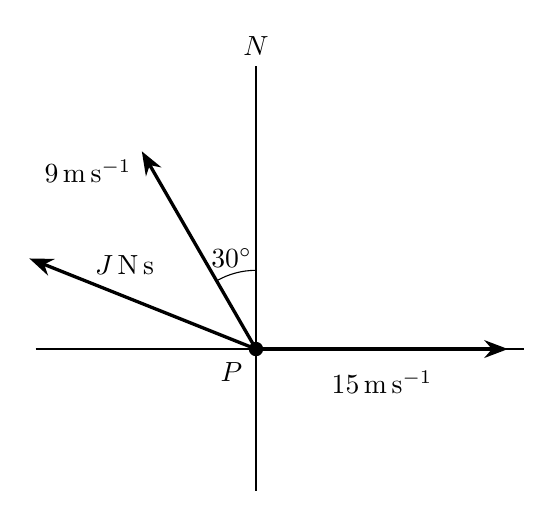
\begin{tikzpicture}[scale=2, >=Stealth]
        \coordinate (P) at (0,0);

        \pgfmathsetmacro{\angV}{120} % bearing 330° = 30° west of north
        \pgfmathsetmacro{\angJ}{180 - atan((9*sin(60))/(15 + 9*cos(60)))}

        \draw[thin] (-1.4,0) -- (1.7,0);
        \draw[thin] (0,-0.9) -- (0,1.8);
        \node[above] at (0,1.8) {$N$};

        \draw[very thick, -{Stealth[length=3mm]}]
            (P) -- (1.6,0)
            node[midway, below=4pt] {$15\,\mathrm{m\,s^{-1}}$};

        \draw[very thick, -{Stealth[length=3mm]}]
            (P) -- (\angV:1.45)
            node[pos=0.9, left=4pt] {$9\,\mathrm{m\,s^{-1}}$};

        \draw[very thick, -{Stealth[length=3mm]}]
            (P) -- (\angJ:1.55)
            node[pos=0.58, above=4pt] {$J\,\mathrm{N\,s}$};

        \fill (P) circle (1.3pt);
        \node[below left=2pt] at (P) {$P$};

        \coordinate (Ndir) at (0,1.5);
        \coordinate (Vdir) at (\angV:1.5);
        \pic[
            draw,
            angle radius=10mm,
            angle eccentricity=1.2,
            "$30^\circ$"
        ] {angle = Ndir--P--Vdir};
    \end{tikzpicture}
\end{figure}


A particle $P$ of mass $0.4\,\mathrm{kg}$ is moving due east with speed $15\,\mathrm{m\,s^{-1}}$ on a smooth horizontal plane. The particle receives a horizontal impulse of magnitude $J\,\mathrm{N\,s}$. \\

Immediately afterwards, $P$ is moving with speed $9\,\mathrm{m\,s^{-1}}$ on a bearing of $330^\circ$, as shown in the diagram. \\

Find the value of $J$ \marks{6}

\newpage

% ---- Question 4 ----
\questionitem
% [Source: _QBT__Vector_Momentum_and_Impulse, Q4]

A particle $Q$ of mass $0.5\,\mathrm{kg}$ is moving on a smooth horizontal surface with speed $10\,\mathrm{m\,s^{-1}}$ in the direction of the vector $4\mathbf{i}-3\mathbf{j}$. The particle then receives an impulse of magnitude $5\,\mathrm{N\,s}$ in the direction of the vector $3\mathbf{i}+4\mathbf{j}$. \\

\begin{enumerate}[label=\textbf{(\alph*)}]
  \item Find the speed of $Q$ immediately after receiving the impulse \marks{4} \\
\end{enumerate}
As a result of receiving the impulse, the direction of motion of $Q$ is turned through an angle $\theta^\circ$. \\
\begin{enumerate}[label=\textbf{(\alph*)}, resume]
  \item Find the value of $\theta$ \marks{2} \\
\end{enumerate}

\newpage

% ---- Question 5 ----
\questionitem
% [Source: _QBT__Vector_Momentum_and_Impulse, Q5]

A particle $P$ of mass $1\,\mathrm{kg}$ is moving with velocity $(3\mathbf{i}+\mathbf{j}+\mathbf{k})\,\mathrm{m\,s^{-1}}$. \\

The particle receives an impulse $\lambda(2\mathbf{i}+\mathbf{j}+2\mathbf{k})\,\mathrm{N\,s}$, where $\lambda$ is a constant. \\

Immediately after receiving the impulse, the kinetic energy of $P$ is $19\,\mathrm{J}$. \\

Find the possible values of $\lambda$ \marks{7}

\newpage

% ---- Question 6 ----
\questionitem
% [Source: _QBT__Vector_Momentum_and_Impulse, Q6]

A particle $P$ of mass $5\,\mathrm{kg}$ is moving with speed $13\,\mathrm{m\,s^{-1}}$ in the direction of the vector $5\mathbf{i}-12\mathbf{j}$ when it receives an impulse $(45\mathbf{i}+90\mathbf{j})\,\mathrm{N\,s}$. \\

\begin{enumerate}[label=\textbf{(\alph*)}]
  \item Find the speed of $P$ immediately after receiving the impulse \marks{4} \\
\end{enumerate}
The direction of motion of $P$ is then changed by $\alpha^\circ$. \\
\begin{enumerate}[label=\textbf{(\alph*)}, resume]
  \item Find the value of $\alpha$ \marks{2} \\
\end{enumerate}

\newpage

% ---- Question 7 ----
\questionitem
% [Source: _QBT__Vector_Momentum_and_Impulse, Q7]

A particle of mass $1\,\mathrm{kg}$ is moving with velocity $(\mathbf{i}+3\mathbf{j}-\mathbf{k})\,\mathrm{m\,s^{-1}}$ when it receives an impulse $\mathbf{I}\,\mathrm{N\,s}$. \\

As a result, its kinetic energy increases by $6.5\,\mathrm{J}$ and the particle then moves in the direction $(\mathbf{i}+2\mathbf{j}+\mathbf{k})$. \\

Find $\mathbf{I}$ \marks{7}

\newpage

% ---- Question 8 ----
\questionitem
% [Source: _QBT__Vector_Momentum_and_Impulse, Q8]

A particle of mass $0.8\,\mathrm{kg}$ is moving with speed $5\,\mathrm{m\,s^{-1}}$ in the direction of the vector $3\mathbf{i}+4\mathbf{j}$. It is then acted on by a constant force of $(8\mathbf{i}-6\mathbf{j})\,\mathrm{N}$ for $0.4\,\mathrm{s}$. \\

\begin{enumerate}[label=\textbf{(\alph*)}]
  \item Find the speed of the particle at the end of the $0.4\,\mathrm{s}$ interval \marks{5} \\
  \item Find the size of the angle between the direction of motion of the particle before the force acts and the direction of motion of the particle at the end of the $0.4\,\mathrm{s}$ interval \marks{3} \\
\end{enumerate}
\end{enumerate}
\end{document}
